\subsection{Gestionar su cuenta y métodos de pago}
\begin{itemize}
    \item Para esto se debe ingresar a “Mi perfil”
    \begin{figure}[H]
        \centering
    
\includegraphics[width=0.8\linewidth]{guiamodulo/navbar-miperfil.png}
    \caption{Barra de navegación, Mi perfil.}
    \label{fig:navbar-miperfil}
    \end{figure}

     \item Alli se puede “Agregar método de pago” o consultar los métodos agregados.
     \begin{figure}[H]
         \centering
     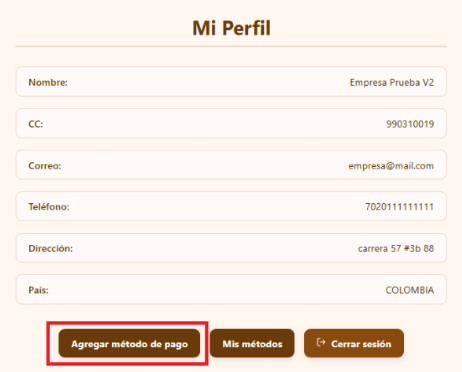
\includegraphics[width=0.6\linewidth]{guiamodulo/perfil-metodopago.png}
     \caption{Perfil, método de pago.}
     \label{fig:perfil-metodopago}
     \end{figure}

     \item Donde puede agregar su método de pago llenando los siguientes campos, y dando click en “Guardar tarjeta”.
     \begin{figure}[H]
         \centering
     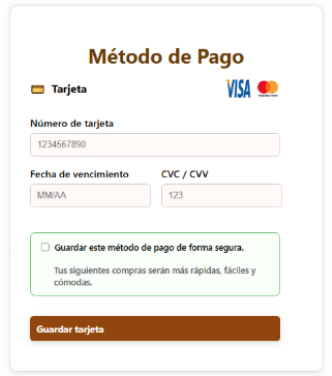
\includegraphics[width=0.5\linewidth]{guiamodulo/metodopago.png}
     \caption{Registrar método de pago.}
     \label{fig:metodopago}
     \end{figure}
\end{itemize}


\subsection{Buscar y registrar dominios}
\begin{enumerate}
\item Para Registrar dominios se debe, en primer lugar, escribir el dominio deseado y dando click en “Buscar Dominio” en la pantalla de inicio vista en la figura \ref{fig:inicio}:

\item Luego se debe “agregar al carrito” el dominio deseado, de la siguiente manera:
    \begin{figure}[H]
        \centering
    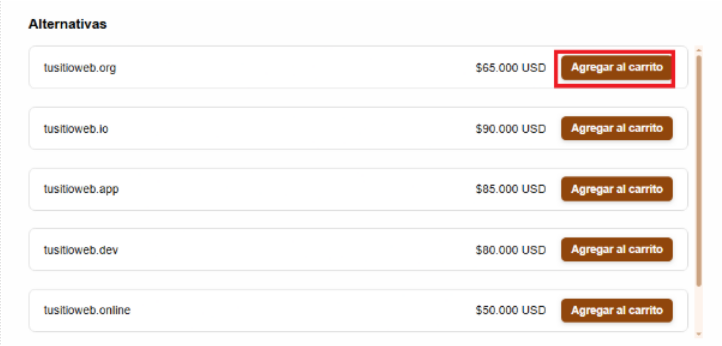
\includegraphics[width=0.8\linewidth]{guiamodulo/domino.png}
    \caption{Resultados a busqueda de un dominio.}
    \label{fig:domino-busqueda}
    \end{figure}
\end{enumerate}

\subsection{Usar el carrito de compras}

\begin{enumerate}
    \item Para usar el carrito de compras, se debe tener ya seleccionados los dominios y se debe dar clic en “Carrito”.
    \begin{figure}[H]
        \centering
    
\includegraphics[width=0.8\linewidth]{guiamodulo/navbar-carrito.png}
    \caption{Barra de navegación, carrito.}
    \label{fig:navbar-carrito}
    \end{figure}

    \item Luego se debe verificar que los dominios sean los deseados y si todo es correcto dar click en “Realizar el pago”
    \begin{figure}[H]
        \centering
    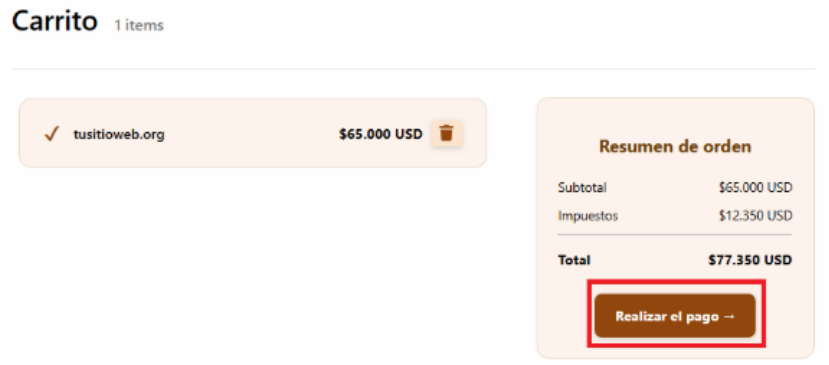
\includegraphics[width=0.8\linewidth]{guiamodulo/carrito-pago.png}
    \caption{Carrito}
    \label{fig:carrito-pago}
    \end{figure}

    \item Donde se recibirá el siguiente mensaje, con copia de su factura a su correo electronico
    \begin{figure}[H]
        \centering
    
\includegraphics[width=0.5\linewidth]{guiamodulo/carrito-aviso.png}
    \caption{Carrito, notificación.}
    \label{fig:carrito-aviso}
    \end{figure}

    \item Ahora, se puede verificar los dominios en la pestaña “Mis dominios”
    \begin{figure}[H]
        \centering
    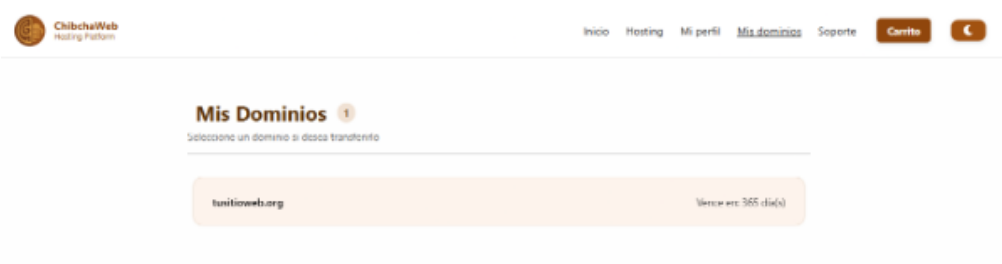
\includegraphics[width=0.8\linewidth]{guiamodulo/domino-usuario.png}
    \caption{Dominios del usuario.}
    \label{fig:domino-usuario}
    \end{figure}

\end{enumerate}
